\section{Methodology}
% TODO1: mention the simulation setting.
% TODO2: key cache error analysis
% TODO3: more details about Table 2


In scenarios with long contexts or batched inferences, the memory and speed bottlenecks are storing and loading KV cache.
The most simple and effective way to alleviate this problem is to reduce the total bytes occupied by KV cache, specifically, quantization.
Following this motivation, we first evaluate the performance of the existing quantization method in Section \ref{sec: quant prelim}.
Our observations suggest that key and value cache should be quantized along different dimensions. We analyze the rationale behind this observation in Section \ref{sec: analysis}.
Then based on the analysis, we propose \kivi{}, a new KV cache quantization method along with its streaming data structure, detailed in Section \ref{sec: algo}.


\subsection{Preliminary Study of KV Cache Quantization}
\label{sec: quant prelim}


As we analyzed in Section \ref{sec: background}, KV cache functions as a streaming data structure, where the new tensor arrives sequentially.
Thus, optimization-based methods like GPTQ \citep{gptq} are unsuitable for quantizing KV cache due to the overhead.
To the best of our knowledge, the most flexible way for quantizing KV cache is the round-to-nearest quantization.
The $B-$bit integer quantization-dequantization process can be expressed as:

\vspace{-2em}
\begin{equation}
    Q(\mX) = \bm\lfloor \frac{\mX - z_X}{s_X} \bm\rceil, ~~~
    \mX' = Q(\mX) \cdot s_X + z_X,  \nonumber
\end{equation}
\vspace{-2em}

\begin{table}
\centering
% \vspace{-1.5em}
\small
\caption{The results of simulated KV cache group-wise quantization with various configurations. The group size is set as 32. $\mathbb{C}$ stands for per-channel quantization and $\mathbb{T}$ stands for per-token quantization. Please check the whole evaluation in Table \ref{tab:merged-lm-eval}.}
\vspace{-.5em}
\label{tab:sub_simulation}
\begin{tabular}{lcc} 
\toprule
\textbf{Llama-2-13B}                         & \multicolumn{1}{l}{\textbf{CoQA}} & \textbf{TruthfulQA}  \\ 
\midrule
16bit                               & 66.37                            & 29.53              \\
4bit (K - $\mathbb{T}$, V - $\mathbb{T}$)     & 66.48                            & 29.51              \\
\midrule
2bit (K - $\mathbb{T}$, V - $\mathbb{T}$)     & 52.93                             & 24.98              \\
2bit (K - $\mathbb{C}$, V - $\mathbb{C}$) & 2.88                            & 0.74               \\
2bit (K - $\mathbb{T}$, V - $\mathbb{C}$)   & 2.80                            & 0.26               \\
2bit (K - $\mathbb{C}$, V - $\mathbb{T}$)   & \textbf{63.53}                             & \textbf{28.60}              \\
\bottomrule
\end{tabular}
% \vspace{-3em}
\end{table}

where $z_X=\min \mX$ is the zero-point, $s_X=(\max \mX - \min \mX)/(2^B - 1)$ is the scaling factor, and $\bm\lfloor\cdot\bm\rceil$ is the rounding operation. 
Here we ignore the batch size for ease of understanding.
As shown in Figure \ref{fig: quant scheme}, $\mX$ is quantized along either the token or channel dimension group-wisely. 

\begin{figure*}[h]
    \centering
    \subfigure{
    \centering
    	\begin{minipage}[t]{0.25\linewidth}
    		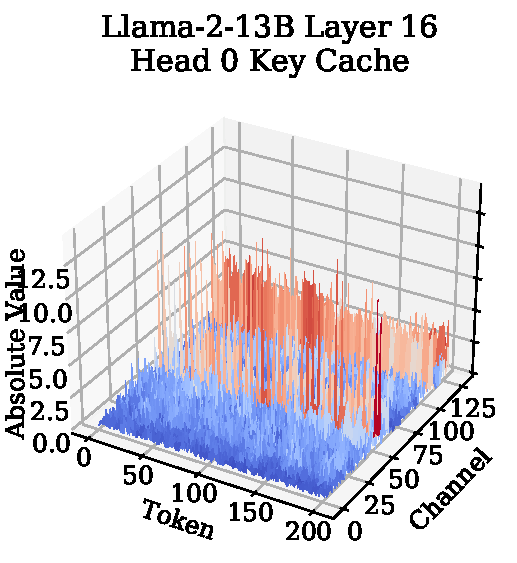
\includegraphics[width=0.99\linewidth]{figures/kvcache_vis/Llama-2-13b-hf_layer16_head0_k.pdf}
    	\end{minipage}%
    }
    \!\!\!\!\!\!
    \subfigure{
    \centering
    	\begin{minipage}[t]{0.25\linewidth}
    		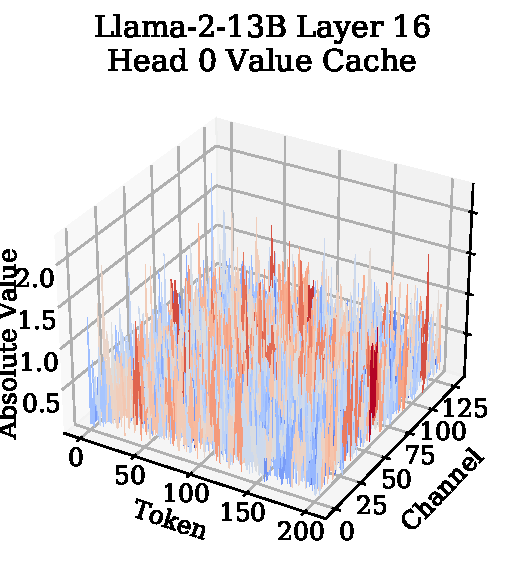
\includegraphics[width=0.99\linewidth]{figures/kvcache_vis/Llama-2-13b-hf_layer16_head0_v.pdf}
    	\end{minipage}%
    }
    \!\!\!\!\!\!
    \subfigure{
    \centering
    	\begin{minipage}[t]{0.25\linewidth}
    		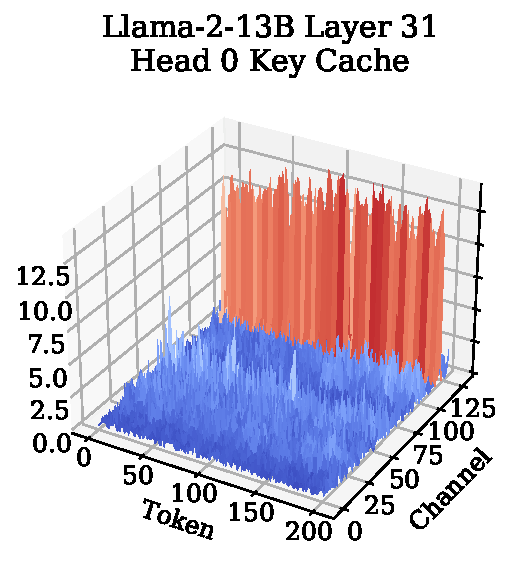
\includegraphics[width=0.99\linewidth]{figures/kvcache_vis/Llama-2-13b-hf_layer31_head0_k.pdf}
    	\end{minipage}
    }
    \!\!\!\!\!\!
    \subfigure{
    \centering
    	\begin{minipage}[t]{0.25\linewidth}
    		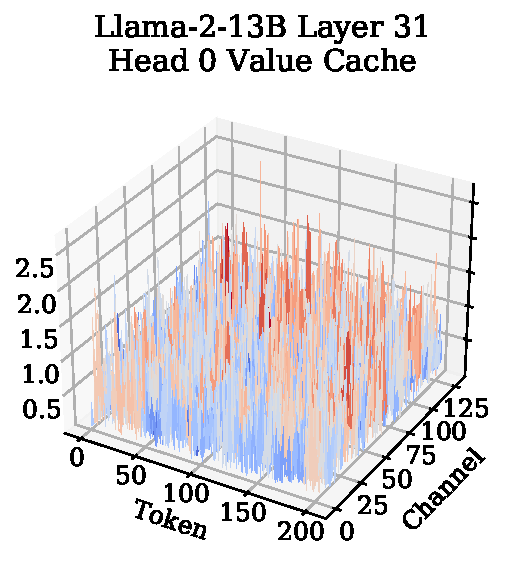
\includegraphics[width=0.99\linewidth]{figures/kvcache_vis/Llama-2-13b-hf_layer31_head0_v.pdf}
    	\end{minipage}
    }
    \!\!\!\!\!\!
    \subfigure{
    \centering
    	\begin{minipage}[t]{0.25\linewidth}
    		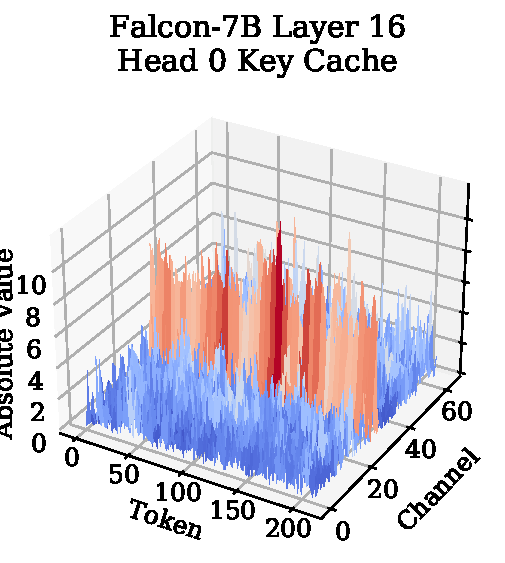
\includegraphics[width=0.99\linewidth]{figures/kvcache_vis/falcon-7b_layer16_head0_k.pdf}
    	\end{minipage}%
    }
    \!\!\!\!\!\!
    \subfigure{
    \centering
    	\begin{minipage}[t]{0.25\linewidth}
    		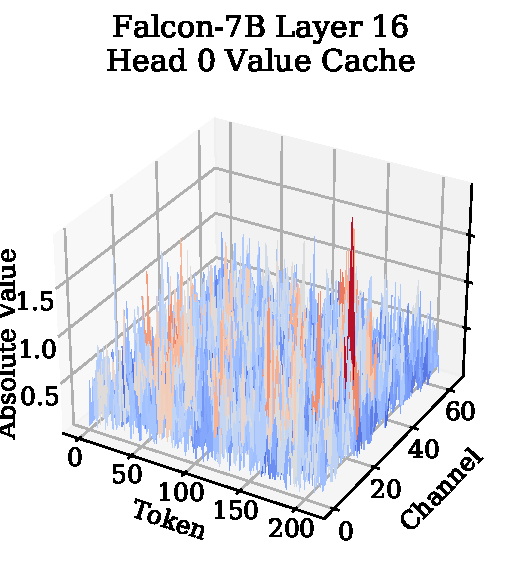
\includegraphics[width=0.99\linewidth]{figures/kvcache_vis/falcon-7b_layer16_head0_v.pdf}
    	\end{minipage}%
    }
    \!\!\!\!\!\!
    \subfigure{
    \centering
    	\begin{minipage}[t]{0.25\linewidth}
    		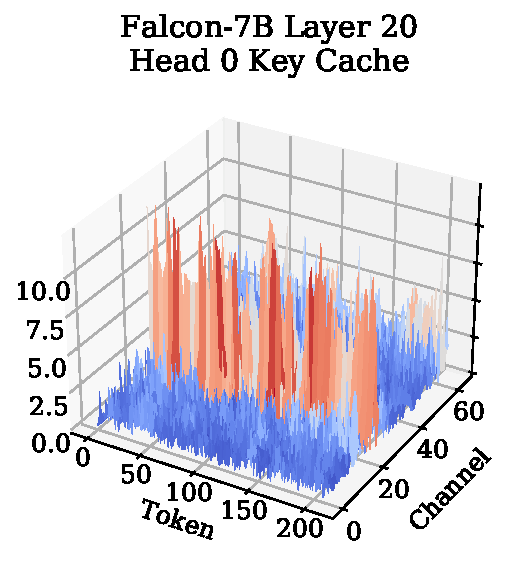
\includegraphics[width=0.99\linewidth]{figures/kvcache_vis/falcon-7b_layer20_head0_k.pdf}
    	\end{minipage}
    }
    \!\!\!\!\!\!
    \subfigure{
    \centering
    	\begin{minipage}[t]{0.25\linewidth}
    		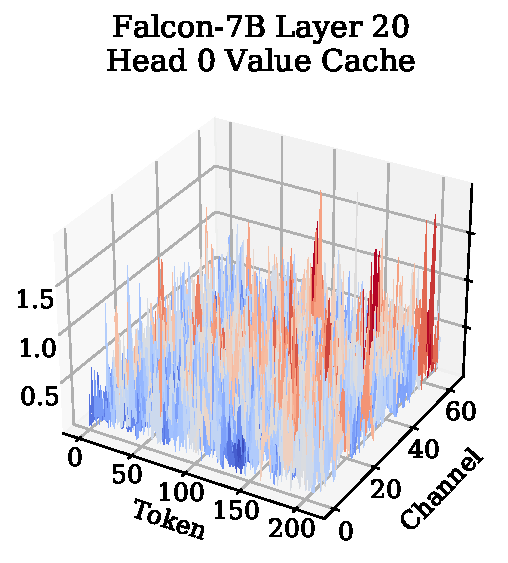
\includegraphics[width=0.99\linewidth]{figures/kvcache_vis/falcon-7b_layer20_head0_v.pdf}
    	\end{minipage}
    }
    \vspace{-1em}
    \caption{Magnitude of key and value cache for Llama-2-13B and Falcon-7B. We observe (1) for key cache, there are a few channels whose magnitudes are very large.
    (2) for value cache, there is no obvious outlier pattern.}
    \label{fig: vis}
\end{figure*}

Considering the streaming nature of KV cache, previous studies often apply per-token quantization to both key and value cache since the newly quantized KV cache can be naively added to the existing quantized one along the token dimension \citep{flexgen}. While per-channel quantization is non-trivial, we have designed a padding method to implement per-channel quantization to explore its effect on both key and value cache.

\paragraph{Setting.}
In Table \ref{tab:sub_simulation}, we show the results of fake KV cache group-wise quantization with different configurations on the Llama-2-13B model for the CoQA and TruthfulQA tasks. We use a group size of 32 for all configurations.
Here fake quantization means we simulate the quantization process by first quantizing KV cache into lower precision and then dequantizing it in the attention layer.
For per-channel quantization, if the number of tokens is not divided evenly into groups, we add zero-padding to ensure it can be grouped perfectly.
In this way, we ensure that all tokens in KV cache are quantized for a fair comparison.
The detailed experimental setting can be found in Section \ref{sec: setting}.
Specifically, we observe that: 

\noindent
\textbf{OB 1.} When using the commonly used per-token quantization to both key and value caches, INT4 precision can maintain accuracy. However, reducing it to INT2 results in a notable accuracy drop.

\noindent
\textbf{OB 2.} When value cache is quantized per-channel, the accuracy significantly worsens regardless of how key cache is quantized.

\noindent
\textbf{OB 3.}  When using a lower numerical precision such as INT2, the most accurate approach is to quantize key cache per-channel and value cache per-token.



\subsection{Why Key and Value Cache Should Quantize Along Different Dimensions?}
\label{sec: analysis}
In Table \ref{tab:sub_simulation}, we observe that quantizing key cache per-channel and value cache per-token to 2bit results in a very small accuracy drop.
Here we analyze why this configuration delivers better accuracy.
In Figure \ref{fig: vis} we visualize the original KV cache distribution at different layers.
We observe that \textbf{in key cache, some fixed channels exhibit very large magnitudes, whereas in value cache, there is no significant pattern for outliers.}

\vspace{-1em}
\noindent
\paragraph{Analysis of Key Cache.}
The above observation for key cache aligns with previous findings that certain fixed columns in activations exhibit larger outliers \citep{llmint8, lin2023awq}.
The persistence of outliers within each channel means that per-channel quantization can confine the quantization error to each individual channel without impacting the other normal channels.
Thus, Figure \ref{fig: vis} explains why key cache should be quantized per-channel. 
In Table \ref{tab: v cache analysis} we show key cache relative reconstruction error $\|\frac{\mX_K-\mX_K'}{\mX_K}\|_F$, along with the relative attention score error $\|\frac{\mA-\mA'}{\mA}\|_F$ where $\mA'=\text{Softmax}(\vt_Q\mX^{'\top}_K)$. 
We observe that the per-token quantization can lead to almost $5\times$ larger attention score error than per-channel quantization, which is consistent with Figure \ref{fig: vis}.

\noindent

\begin{table}[h]
\centering
\small
% \vspace{-1em}
\caption{The relative error statistics averaged over all layers and all heads}
% \vspace{-1em}
\label{tab: v cache analysis}
\begin{tabular}{lcc} 
\toprule
  Llama-2-13B                 & K Per-Token & K Per-Channel  \\
  \midrule
Avg. $\|\frac{\mX_K-\mX_K'}{\mX_K}\|_F$          & 13.67       & 4.55           \\[2pt]
Avg. $\|\frac{\mA-\mA'}{\mA}\|_F$          & 47.00       & 9.60           \\[2pt]
Attention sparsity & \multicolumn{2}{c}{84.3\%}   \\
\bottomrule
\toprule
      & V Per-Token & V Per-Channel  \\ 
\midrule
Avg. $\|\frac{\mX_V-\mX_V'}{\mX_V}\|_F$           & 4.57       & 3.73           \\[2pt]
Avg. $\Delta$   & 3.55        & 49.89          \\ 
\bottomrule
\end{tabular}
\end{table} 

\begin{figure*}[t!]
    \centering
    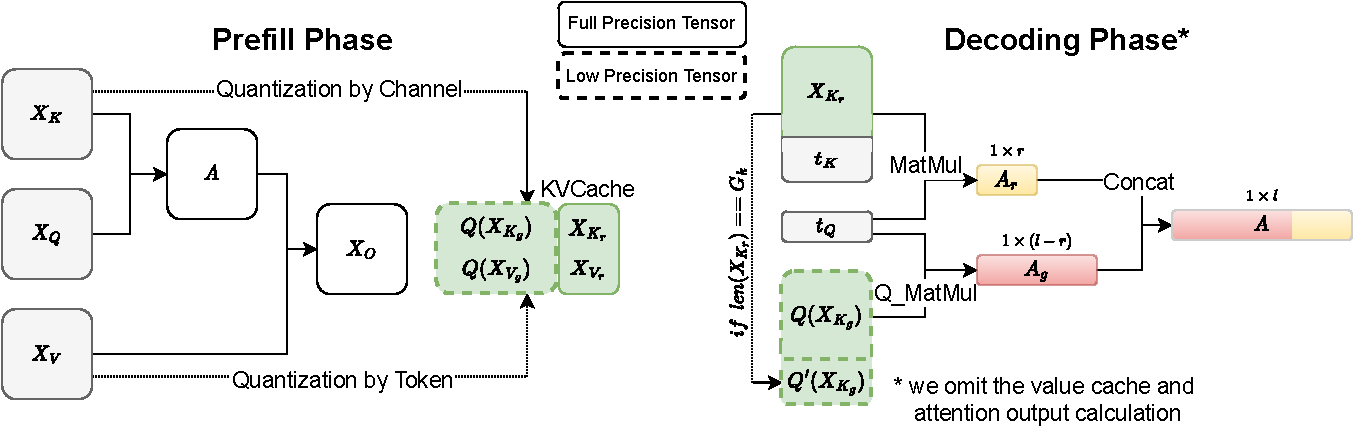
\includegraphics[width=0.9\textwidth]{figures/kivi_algo_v3.pdf}
    \vspace{-1em}
    \caption{The overview of \kivi{} algorithm. For ease of illustration, we omit the value cache and attention output parts. The detailed pseudo-code is provided in Algorithm \ref{algo: kivi}.
    Here ``Q\_Matmul'' is the mix-precision matrix multiplication which fuses the dequantization with matrix multiplication at the tiling level.}
    \label{fig: kivi}
    \vspace{-1em}
\end{figure*}

\paragraph{Analysis of Value Cache.}
Unlike key cache, value cache does not show the channel-wise outlier pattern. Furthermore, Figure \ref{fig: vis} alone cannot explain \textbf{OB2}, which indicates value cache should only be quantized per-token. 
This is because Figure \ref{fig: vis} implies that errors should be comparable for both per-token and per-channel quantization, given the absence of a clear pattern.
As shown in \Eqref{eq: av}, value cache is used to calculate the attention output $\vt_O$.
Instead of analyzing the quantization error of value cache $\mX_V$, in Table \ref{tab: v cache analysis} we analyze the relative error $\Delta=\|\frac{\mA\mX_V-\mA \mX'_V}{\mA\mX_V}\|_F$ with different quantization configurations.
Surprisingly, we observe that the per-token quantization error is almost $15\times$ smaller than per-channel quantization, which explains why \textbf{OB2} happens.
The intuition behind this observation stems from the attention sparsity.
\Eqref{eq: av} can be written as:

\vspace{-2em}
\begin{align}
    [\mA \mX_V]_{i*} = \sum_{j=1}^{l_{\text{prompt}}} \mA_{ij} [\mX_{V}]_{j*},
    \label{eq: att}
\end{align}
\vspace{-2em}

where $[\mX_{V}]_{j*}$ is the $j$-th row of $\mX_{V}$.
From \Eqref{eq: att}, the attention output is the weighted summation of value cache across various tokens, with the weights being the attention scores.
Since the attention score is highly sparse \citep{tian2023scan}, the output is just the combination of value caches of a few important tokens.
The per-token quantization can confine the error to each individual token.
Thus, quantizing other tokens does not affect the accuracy of important tokens. Consequently, per-token quantization leads to a much smaller relative error $\Delta$. 

\subsection{\kivi{}: Algorithm and System Support}
\label{sec: algo}

\paragraph{Algorithm.}
As we previously analyzed, key cache should be quantized per-channel and value cache should be quantized per-token.
Recall that key and value cache of newly generated tokens arrive sequentially.
From the implementation perspective, per-token quantization aligns well with streaming settings, allowing newly quantized tensors to be directly appended to the existing quantized value cache by token dimension.
However, for per-channel quantization, the quantization process spans across different tokens, which cannot be directly implemented in the streaming setting.
As shown in Figure \ref{fig: kivi}, our key idea to solve this problem is to group key cache every $G$ tokens and quantize them separately. 
Because the number of tokens in $\mX_K$ can be arbitrary, we split $\mX_K$ into two parts, namely, the grouped part $\mX_{K_g}=\mX_{K}[:l-r]$ and residual part $\mX_{K_r}=\mX_{K}[l-r:]$, where $l$ is the number of tokens inside the current key cache $\mX_K$, $r$ is the number of residual tokens, where $l-r$ can be divisible by $G$.

Since $\mX_{K_g}$ can be evenly divided into $(l-r)/G$ groups, we only store $Q(\mX_{K_g})$ with group-wise quantization, while $\mX_{K_r}$ is kept in full precision.
During the decoding process, each newly arrived key cache $\vt_K$ is added to $\mX_{K_r}$ and once $\mX_{K_r}$ reaches $R$ tokens, which is a hyperparameter - residual length, we quantize and concatenate it with the previously quantized $Q(\mX_{K_G})$. 
Then we reset $\mX_{K_r}$ to an empty tensor. We note that $R$ should be divisible by $G$.
With tiled matrix multiplication, the raw attention logits is then calculated as:

\vspace{-2em}
\begin{align}
\mA_g &= \vt_Q Q(\mX^{\top}_{K_g}), \nonumber \\
\mX_{K_r} &= \text{Concat}([\mX_{K_r}, \vt_K]), \nonumber \\
\mA_r &= \vt_Q \mX^{\top}_{K_r}, \nonumber \\
\mA &= \text{Concat}([\mA_g, \mA_r]).
\label{eq: attquant}
\end{align}
\vspace{-2em}

% \begin{align}
% \vt_Q \mX^{\top}_K= \text{Concat}([\vt_Q Q(\mX^{\top}_{K_g}), \vt_Q \mX^{\top}_{K_r}]).
% \label{eq: attquant}
% \end{align}

For value cache, similar to key cache, we also split it into two parts and keep the most recent value cache in full precision, namely, $\mX_{V_g}$ and $\mX_{V_r}$. Specifically, we maintain a queue and each newly arrived value cache is pushed into the queue. 
Once the queue reaches the predefined residual length $R$, the most outdated value cache is poped. Then the poped value cache is quantized per-token and concatenated with the previously quantized value cache along the token dimension. 

As shown in Figure \ref{fig: kivi}, we also emphasize that during the prefill phase, the exact key and value tensors are passed to the next layers, although only the quantized KV cache is retained in memory.
The whole algorithm can be found in Appendix \ref{app: implement} Algorithm \ref{algo: kivi}.

\paragraph{Analysis.}
In \kivi{}, the grouped key cache $\mX_{K_g}$ and value cache $\mX_{V_g}$ is quantized, while the residual key cache $\mX_{K_r}$ and value cache $\mX_{V_r}$ is kept in full precision.
By design, there are at most $R$ tokens inside $\mX_{K_r}$ or $\mX_{V_r}$. In practice, we set $R \leq 128$ and the sequence length $l_{\text{prompt}}+l_{\text{gen}}$ is often much longer than $R$.
Thus the memory overhead from $\mX_{K_r}$ and $\mX_{V_r}$ is negligible when considering the benefit from extreme low-bit quantization, especially for the long context scenarios.
Also, since the newly arrived key and value tensors are added to $\mX_{K_r}$ and $\mX_{V_r}$ in full precision, \kivi{} maintains a full precision KV cache sliding window for the local relevant tokens.
This window size is expected to be $\frac{R}{2}$ for key cache, and $R$ for value cache.
\textbf{Later in the experiment section, we show that this full precision sliding window is crucial for obtaining desirable performance on hard tasks, such as GSM8K.}

\paragraph{System Support.}
We provide a hardware-friendly implementation for running \kivi{} on GPUs.
To minimize the overhead, we have fused the dequantization process with matrix multiplication, e.g., Q\_MatMul in Figure \ref{fig: kivi}, using CUDA. 
We also implement the group-wise quantization kernel in Triton.
Our method is fully compatible with weight-only quantization.
